
%!TEX TS-program = xelatex
\documentclass[spanish]{friggeri-cv}
\usepackage[spanish]{babel}
\selectlanguage{spanish}
\usepackage[utf8]{inputenc}
\usepackage{afterpage}
\usepackage{hyperref}
\usepackage{color}
\usepackage{xcolor}
\usepackage[skins]{tcolorbox}
\hypersetup{
    pdftitle={},
    pdfauthor={},
    pdfsubject={},
    pdfkeywords={},
    colorlinks=false,       % no lik border color
   allbordercolors=white    % white border color for all
}
\RequirePackage{xcolor}
\definecolor{pblue}{HTML}{0395DE}

\begin{document}
\header{Lo\"{i}c}{Dutrieux}
      {Especialista de Geo-Información}
      
% Fake text to add separator      
\fcolorbox{white}{gray}{\parbox{\dimexpr\textwidth-2\fboxsep-2\fboxrule}{%
.....
}}

% In the aside, each new line forces a line break
\begin{aside}
% TODO: Age, nationality could also be added here
    ~
    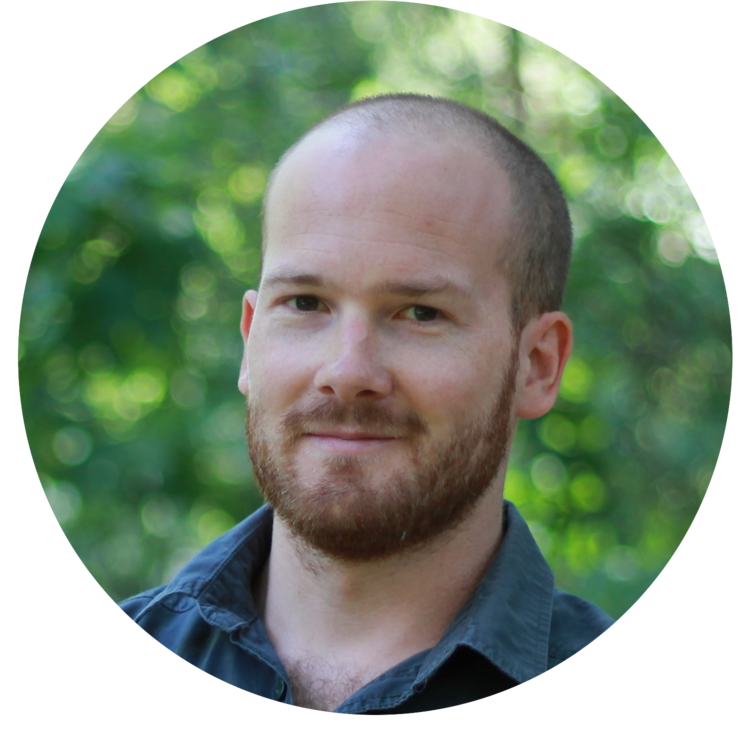
\includegraphics[width=2.5cm]{img/profile_circle_small.png}
    ~
  \section{Nacionalidad}
    Francés
    ~
  \section{Estado civil}
    Soltero
    ~
  \section{Dirección}
    Dr Nabor Carrillo 127 Casa G
    01780 Olivar de los Padres
    Alvaro Obregon, Ciudad de México, México
    ~
  \section{Tel \& Skype}
    +52 557 854 8336
    loic.dutrieux
    ~
  \section{Correo electrónico}
    \href{mailto:loic.dutrieux@gmail.com}{\textbf{loic.dutrieux@}\\gmail.com}
    ~
  \section{Web}
    \href{http://www.loicdutrieux.net}{loicdutrieux.net}
    % \href{https://www.linkedin.com/in/loicdutrieux}{linkedin.com/in/loicdutrieux}
    \href{https://github.com/loicdtx}{github.com/loicdtx}
    ~
  \section{Programación}
    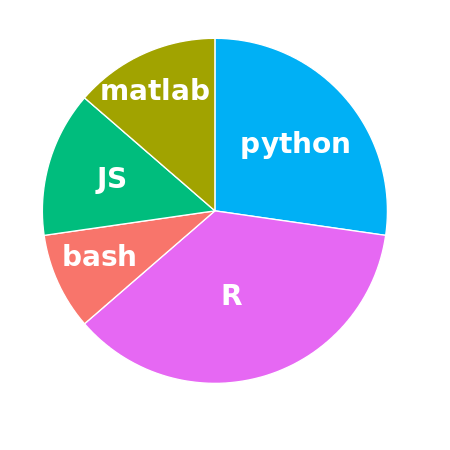
\includegraphics[width=3.5cm]{img/programming.png}
    ~
  \section{Herramientas y Software}
  % TODO: OTB?
    \textbf{Linux}
\includegraphics[scale=0.40]{img/4stars.png}
    \textbf{Git}
\includegraphics[scale=0.40]{img/4stars.png}
    \textbf{QGIS}
\includegraphics[scale=0.40]{img/4stars.png}
    \textbf{GDAL}
\includegraphics[scale=0.40]{img/4stars.png}
    ~
\end{aside}

% TODO: Would be nice to start here with a profile section section: a 4 lines description of who I am and what are my interests 

\section{Experiencia}
\begin{entrylist}
  \entry
    {02/12 - 06/16}
    {Estudiante de doctorado - Investigador}
    {Universidad de Wageningen, Países Bajos}
    {Investigación sobre dynamicas de la selva Amazónica con series de tiempo de imagen satelitales, desarrollo de herramientas para análisis espacial, enseñanza, gestión de proyectos.\\}
 
\end{entrylist}

\section{Educación}
\begin{entrylist}
  \entry
    {2011 - 2016}
    {Doctorado}
    {Universidad de Wageningen, Países Bajos}
    {Percepción remota, análisis de series de tiempo, ecología, desarrollo de algoritmo\\}

  \entry
    {2009 - 2011}
    {MSc \emph{International Land and Water Management}}
    {Universidad de Wageningen, Países Bajos}
    {Temas principales: Sistemas de riego, hidrológica, administración del agua, sociología del desarrollo \\
    Major tesis sobre \emph{Mapping water productivity of rice using remote sensing}\\
    Minor tesis sobre \emph{Vegetation dynamics in the Arctic from Moderate resolution remote sensing time-series}\\}
  \entry
    {2007 - 2011}
    {Maestría en Medio Ambiente y Ingeniería Agrícola}
    {\emph{Ecole Supérieure d'Agriculture d'Angers, France}}
    {Temas principales: Agronomía, Ecología del paisaje, Análisis Espacial, geopolítica, Gestión y Marketing}
  \entry
    {2005 - 2007}
    {DUT (\textit{Licenciatura Profesional Francés}) Biología y Ingeniería del Medio Ambiente}
    {IUT de Digne-Les-Bains, Francia}
    {Temas principales: Hidrobiología, Gestión de aguas residuales, Termodinámica}
\end{entrylist}

\section{Proyectos de código abierto}
    \textbf{bfastSpatial}: \textit{Set of utilities and wrappers to perform change detection on satellite image time-series (Landsat and MODIS)}\\
    \\
    \href{http://geoscripting-wur.github.io/}{\textbf{GeoScripting}}: Curso de maestría sobre uso de programación para ciencias geo-espaciales, enseñado en al Universidad de Wageningen\\
    \\
    Contribuyente regular de la lista de envío \href{https://stat.ethz.ch/mailman/listinfo/r-sig-geo}{R-SIG-Geo}

\pagebreak

% TODO: \section{Self taught subjects}
\section{Honores y premios}
    \textbf{Oustanding Student Paper Award of the American Geophysical Union (AGU)}\\
    San Francisco, Diciembre 2015

\section{Trabajo científico}
    Dutrieux, L. P., Jakovac, C., Latifah, S., Kooistra, L. (2016)\\
    \textbf{Reconstructing land use history from Landsat time-series. Case study of a swidden agriculture system in Brazil}\\
    \textit{International Journal of Applied Earth Observation and Geoinformation}\\
    \\
    Dutrieux, L. P., Verbesselt, J., Kooistra, L., Herold, M. (2015)\\
    \textbf{Monitoring forest cover loss using multiple data streams, a case study of a tropical dry forest in Bolivia.}\\
    \textit{ISPRS Journal of Photogrammetry and Remote Sensing}\\
    \\
    Dutrieux, L. P., Bartholomeus, H., Herold, M., Verbesselt, J. (2012)\\
    \textbf{Relationships between declining summer sea ice, increasing temperatures and changing vegetation in the Siberian Arctic tundra from MODIS time series (2000–11).}\\
    \textit{Environmental Research Letters}\\
    \\
    Dutrieux, L. P., Poorter, L., Equihua, J., Ascarrunz, N., Herold, M., Pe\~{n}a-Claros, M., Roerink, G., Toledo, M., Kooistra, L. (\textit{in review})\\
    \textbf{Country wide mapping of forest diversity and structure by combining forest inventories with remote sensing.}\\
    \\
    Dutrieux, L. P., Kooistra, L., Herold, M., Poorter, L. (\textit{in prep})\\
    \textbf{Post-disturbance recovery in forest spectral properties across the Amazon.}\\
    \\

\begin{aside}
~
~
~
\section{Habilidades Personales}
    % 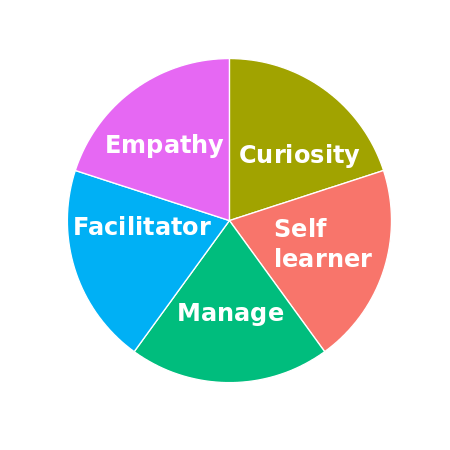
\includegraphics[width=3.5cm]{img/personal.png}
    \textbf{Empatía}
    \textbf{Curiosidad}
    \textbf{Autodidacto}
    \textbf{Manager}
    \textbf{Facilitador} 
    ~
  \section{Lugares donde he vivido}
    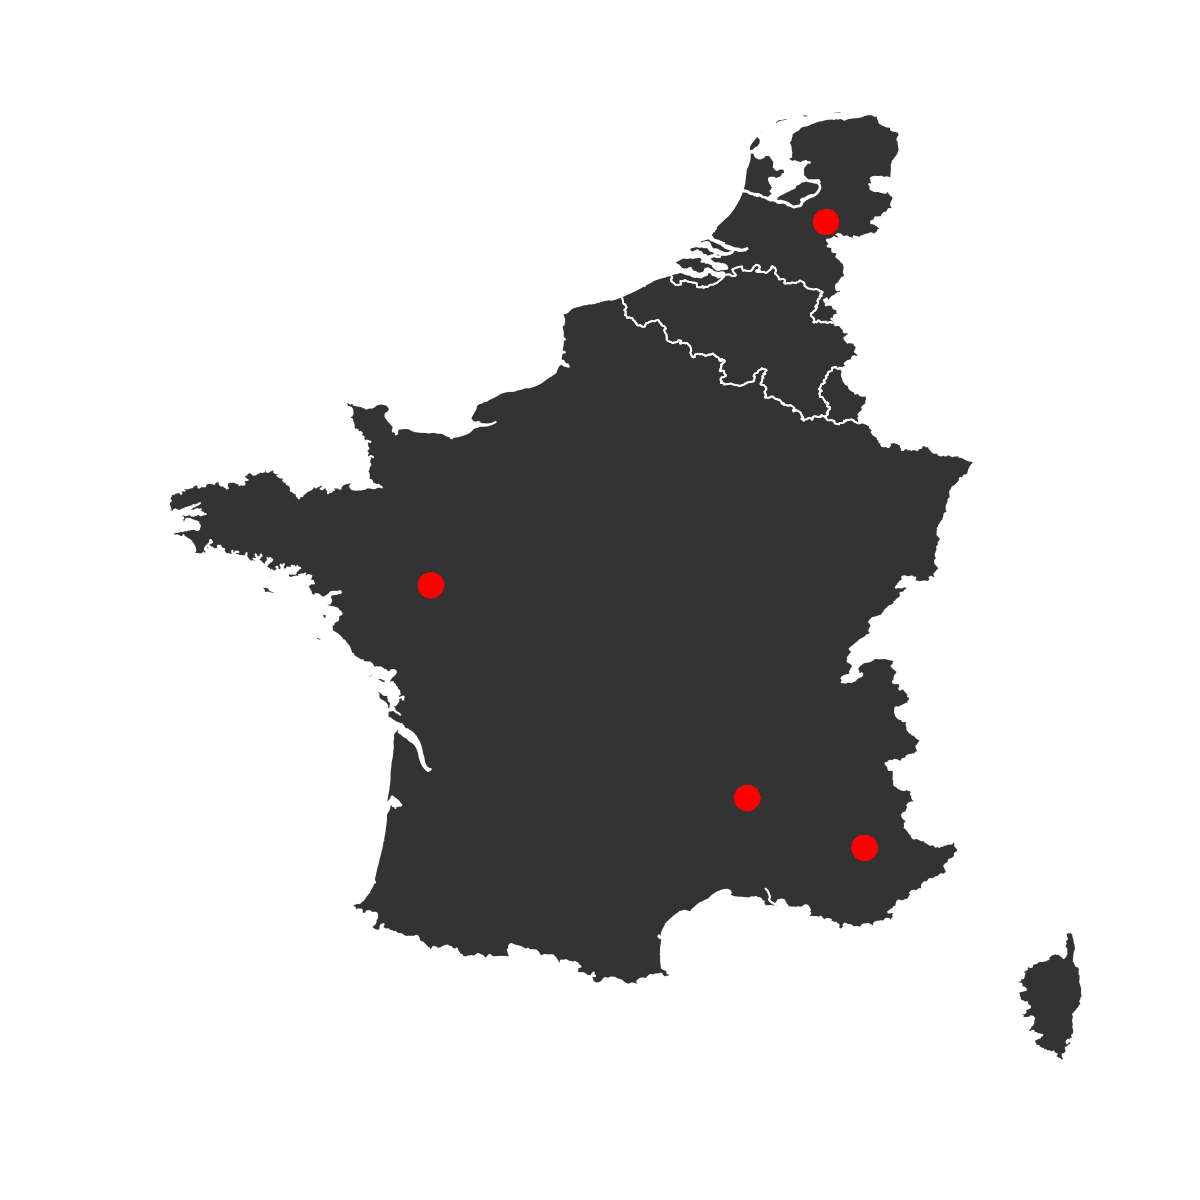
\includegraphics[width=3.5cm]{img/map.png}
    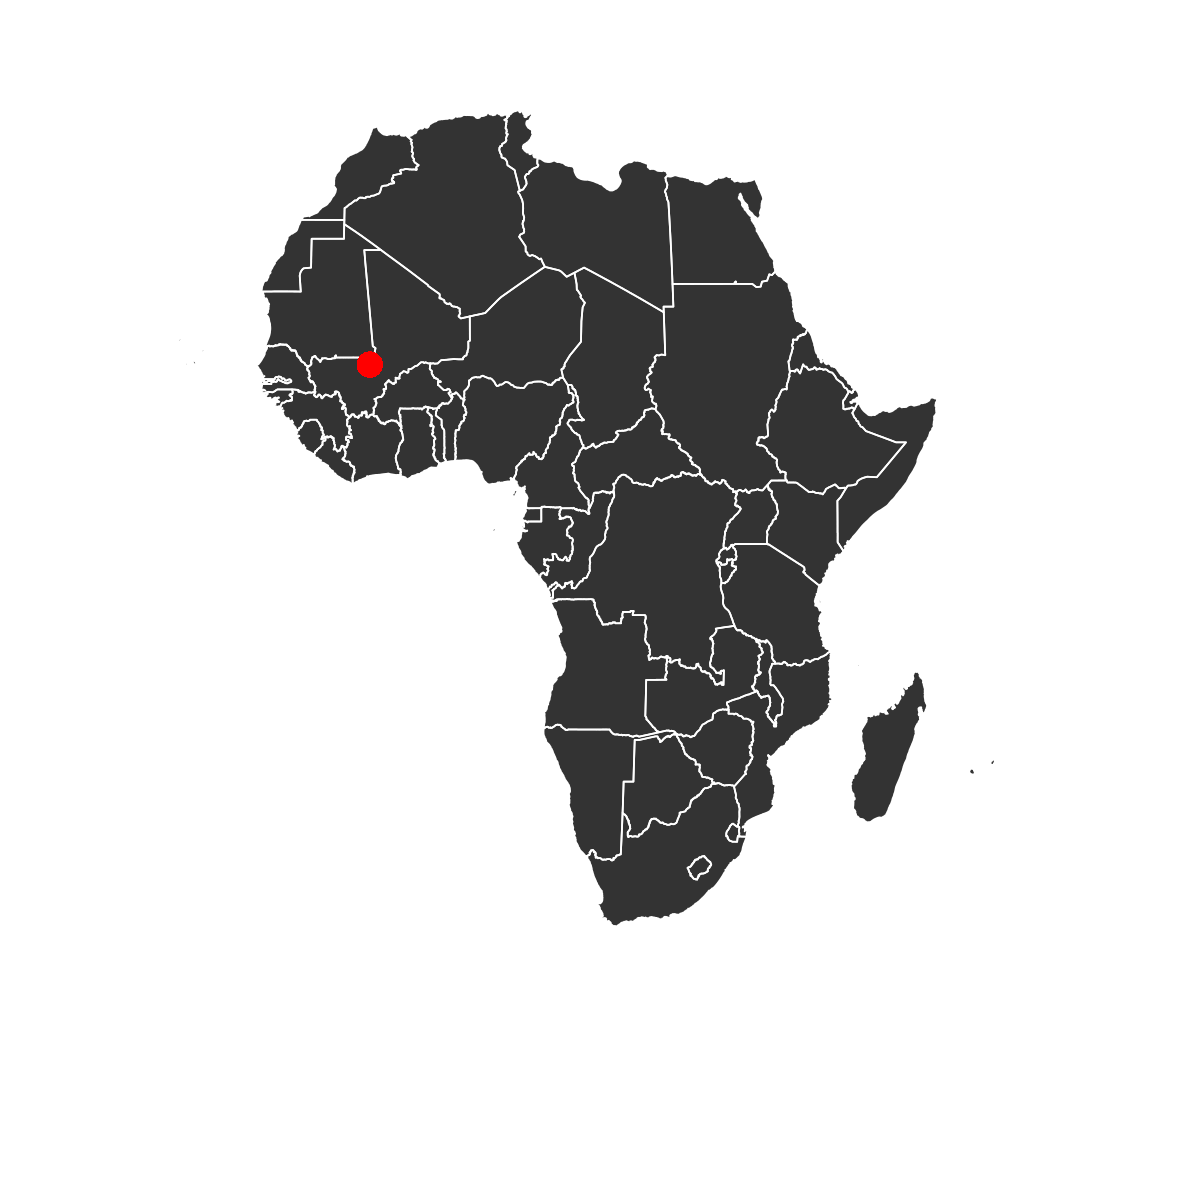
\includegraphics[width=3.5cm]{img/mapAfrica.png}
    ~
  \section{Idiomas}
    \textbf{Ingles}
\includegraphics[scale=0.40]{img/4stars.png}
    \textbf{Francés}
\includegraphics[scale=0.40]{img/5stars.png}
    \textbf{Español}
\includegraphics[scale=0.40]{img/2stars.png}
\end{aside}

\begin{flushleft}
\emph{Febrero 28, 2017}
\end{flushleft}
\begin{flushright}
\emph{Lo\"{i}c Dutrieux}
\end{flushright}

\end{document}
